\documentclass[10pt,twocolumn]{article}

% ------------------------------------------------------------------
% Packages
% ------------------------------------------------------------------
\usepackage[utf8]{inputenc}
\usepackage[T1]{fontenc}
\usepackage{lmodern}
\usepackage{amsmath,amssymb}
\usepackage{graphicx}
\usepackage{booktabs}
\usepackage{array}
\usepackage{multirow}
\usepackage{microtype}
\usepackage{xcolor}
\usepackage{algorithm}
\usepackage{algpseudocode}
\usepackage[hidelinks]{hyperref}
\usepackage[margin=0.8in]{geometry}
\usepackage{tikz}
\usetikzlibrary{arrows.meta,positioning,fit,backgrounds}
\usepackage{enumitem}
\setlist{nosep,leftmargin=1.2em}

\definecolor{accent}{HTML}{2563EB}
\newcommand{\db}{\,\text{dB}}
\newcommand{\mmhg}{\,\text{mmHg}}

\title{\textbf{A Clinically Grounded, Uncertainty-Aware Decision-Support System for
Glaucoma Staging and Screening from Tabular and Fundus Data}}

\author{%
  \normalsize Anonymous Author(s)\\
  \normalsize \textit{Department of Biomedical Informatics}\\
  \normalsize \texttt{corresponding@example.org}
}
\date{}

\begin{document}
\maketitle

% ==================================================================
\begin{abstract}
We present an open, reproducible decision-support system for glaucoma that is
engineered for \emph{clinical validity} first and architectural novelty second.
The system couples two complementary models: (i)~a tabular Transformer that stages
disease severity from $23$ structured ophthalmic and systemic measurements, and
(ii)~a convolutional network that screens color fundus photographs for referable
glaucoma and estimates the vertical cup-to-disc ratio (CDR). Severity labels are
\emph{derived from} the Hodapp--Parrish--Anderson (HPA) staging rules on the
visual-field mean deviation (MD) combined with structural gates on CDR, retinal
nerve-fiber-layer (RNFL) thickness and pattern standard deviation (PSD), rather than
sampled arbitrarily. Predictive uncertainty is quantified with $50$-sample
Monte-Carlo (MC) dropout, decomposed into epistemic and aleatoric parts, and surfaced
as an explicit reliability flag with calibration reported by expected calibration
error (ECE). Disease trajectory is projected with a transparent, EMGT/CIGTS-consistent
closed-form model, and treatment guidance follows stage-dependent target-IOP practice
framed as decision support, not prescription. On a held-out test set
($N{=}600$) the staging model attains accuracy $0.843$, macro-$F_1$ $0.810$,
ROC-AUC $0.954$, Brier score $0.051$ and ECE $0.108$, with per-class $F_1$ from
$0.61$ (mild) to $0.90$ (severe). The fundus screener, trained on the public ACRIMA
set ($705$ images), reaches validation ROC-AUC $1.00$ with CDR mean-absolute-error
(MAE) $\approx 0.10$, and its Grad-CAM saliency localizes the optic disc and cup. We
release the data generator, training scripts, trained weights, a FastAPI service and
a minimal clinical dashboard. \textbf{This is a research and education artifact, not
a medical device, and must not be used for patient care.}
\end{abstract}

% ==================================================================
\section{Introduction}
Glaucoma is a leading cause of irreversible blindness; its clinical management turns
on two recurring questions: \emph{how advanced is the optic neuropathy?} and
\emph{is the intraocular pressure (IOP) low enough to protect the remaining visual
field?} Many machine-learning systems for glaucoma optimize predictive metrics while
embedding assumptions that are clinically indefensible: fabricating a temporal axis
from cross-sectional data, recommending ``treatment'' through adversarial games with
no guideline basis, evolving opaque high-dimensional ``digital-twin'' states, or
emitting confident predictions from image heads that were never trained. Such systems
can look sophisticated and behave unsafely.

This paper deliberately inverts those priorities. We begin from the measurements
clinicians use, label severity with the rule set clinicians apply (HPA), quantify and
\emph{display} uncertainty, and keep every downstream recommendation transparent and
explicitly advisory. We also document a subtle but decisive training pathology---an
unbounded aleatoric loss term---whose correction nearly doubled accuracy, as a
cautionary, reproducible case study. Concretely, our contributions are:

\begin{itemize}
  \item A \textbf{measurement-driven data model} in which severity is a
  deterministic HPA function of the inputs (Section~\ref{sec:data}), eliminating the
  circularity of sampling a class and synthesizing features around it.
  \item A \textbf{tabular Transformer} with per-feature tokenization, learned
  missingness tokens (no imputation), and joint epistemic/aleatoric uncertainty
  (Section~\ref{sec:tabular}).
  \item A \textbf{transparent progression model} and a \textbf{guideline
  decision-support module} that replace opaque and game-theoretic components with
  interpretable, literature-consistent rules (Section~\ref{sec:downstream}).
  \item A \textbf{clinically honest fundus screener}: referable-glaucoma
  classification on real expert labels plus a CDR regressor, with Grad-CAM attribution
  and an explicit ``uncalibrated'' state (Section~\ref{sec:fundus}).
  \item A reproducible \textbf{end-to-end system} and a detailed empirical study with
  per-class, calibration and ablation analyses (Section~\ref{sec:results}).
\end{itemize}

% ==================================================================
\section{Related Work}
\textbf{Glaucoma staging.} The HPA scheme grades severity from the Humphrey
visual-field MD: mild ($\mathrm{MD}>-6\db$), moderate ($-12\le\mathrm{MD}\le-6\db$),
severe ($\mathrm{MD}<-12\db$), corroborated structurally by the vertical CDR and RNFL
thickness. The EMGT, CIGTS and AGIS trials established that IOP reduction slows
progression and underpin stage-dependent target pressures and the
observation\,$\rightarrow$\,medication\,$\rightarrow$\,laser\,$\rightarrow$\,surgery
ladder.

\textbf{Tabular deep learning.} Attention-based encoders with per-feature
tokenization are competitive on heterogeneous clinical tables; we adopt a CLS-token,
pre-layer-norm design.

\textbf{Uncertainty and explainability.} MC dropout approximates the Bayesian
posterior predictive distribution at inference; combined with a learned aleatoric
head and ECE it yields actionable confidence. Attention/SHAP attributions and
Grad-CAM provide feature- and pixel-level explanations.

\textbf{Fundus datasets.} Public corpora include REFUGE, ORIGA, G1020, RIM-ONE~DL and
ACRIMA. We adopt ACRIMA ($396$ glaucoma / $309$ normal) for its permissive,
credential-free distribution and expert binary annotation.

% ==================================================================
\section{Data}
\label{sec:data}

\subsection{Feature schema}
Each encounter comprises $23$ predictors and one target, summarized in
Table~\ref{tab:features}. Features span demographics, bilateral IOP, optic-nerve
structure (CDR, RNFL sectors), visual-field function (MD, PSD, acuity) and systemic
risk factors. The target $y$ is the five-level severity stage.

\begin{table*}[t]
\centering
\caption{Feature dictionary for the tabular model ($23$ predictors $+$ target).}
\label{tab:features}
\small
\begin{tabular}{lllp{0.46\textwidth}}
\toprule
Group & Features & Type & Clinical role \\
\midrule
Demographic & age, sex, ethnicity, eye\_color & num/bin/cat & Baseline risk; age and ancestry modulate prevalence. \\
Pressure & iop\_od, iop\_os & numeric & Primary modifiable risk factor (per eye). \\
Structure & cup\_disc\_ratio, rnfl\_superior, rnfl\_inferior, rnfl\_average & numeric & Optic-nerve damage; larger CDR and thinner RNFL indicate neuropathy. \\
Function & mean\_deviation\_od/os, pattern\_sd, va\_od, va\_os & numeric & Visual-field loss; MD bands drive HPA staging. \\
Systemic & bmi, hba1c, systolic\_bp, diastolic\_bp, diabetes, hypertension, family\_history & num/bin & Comorbid and hereditary risk. \\
Management & treatment & categorical & Current therapy (observation\dots surgery). \\
\midrule
\textbf{Target} & disease\_severity & 5-class & Normal, Suspect, Mild, Moderate, Severe. \\
\bottomrule
\end{tabular}
\end{table*}

\subsection{Generative model and rule-derived labels}
We synthesize $N{=}4000$ encounters. A latent optic-nerve-damage factor
$d\sim\mathrm{Beta}(1.6,3.0)$ (right-skewed, mean $\approx0.35$) drives correlated
structure and function:
\begin{align}
\mathrm{CDR} &\sim \mathcal{N}(0.30+0.55\,d,\;0.07^2),\\
\mathrm{RNFL}_{\text{avg}} &\sim \mathcal{N}(115-60\,d,\;8^2),\\
\mathrm{MD} &\sim \mathcal{N}(-0.5-24\,d^{1.6},\;1.8^2),\\
\mathrm{PSD} &\sim \mathcal{N}(1.6+9\,d,\;1.0^2),\\
\mathrm{IOP} &\sim \mathcal{N}(15.5+8\,d,\;4^2).
\end{align}
Sectoral RNFL, the contralateral eye, acuity and systemic variables follow analogous
conditionals with clinically realistic couplings (e.g.\ diabetes probability rises
with BMI; family-history probability rises with $d$). The severity label is then
\emph{derived} from the realized measurements by Algorithm~\ref{alg:hpa}: a structural
gate establishes glaucomatous versus suspect status, and the worse-eye MD assigns
mild/moderate/severe by the HPA bands. We add $6\%$ adjacent-stage label noise to
emulate inter-grader disagreement and inject missingness on the same fields and at
the rates seen in real clinics (e.g.\ $12\%$ HbA1c, $10\%$ MD, $7$--$8\%$ RNFL/PSD).
The resulting distribution (Table~\ref{tab:classdist}) is screening-skewed toward
``Suspect'', and feature means are monotone across stages
(Table~\ref{tab:monotone}).

\begin{algorithm}[t]
\caption{HPA-based severity labelling (worse-eye MD)}
\label{alg:hpa}
\begin{algorithmic}[1]
\State $g \gets (\mathrm{CDR}\!\ge\!0.70)\lor(\mathrm{RNFL}\!<\!80)\lor(\mathrm{PSD}\!\ge\!5)$
\State $s \gets (\mathrm{CDR}\!\ge\!0.60)\lor(\mathrm{RNFL}\!<\!90)\lor(\mathrm{PSD}\!\ge\!3)$
\If{$g \wedge (\mathrm{MD}\le-3)$}
  \If{$\mathrm{MD}<-12$} \State \Return \textsc{Severe}
  \ElsIf{$\mathrm{MD}\le-6$} \State \Return \textsc{Moderate}
  \Else \State \Return \textsc{Mild} \EndIf
\ElsIf{$s \vee (-6<\mathrm{MD}\le-2)$} \State \Return \textsc{Suspect}
\Else \State \Return \textsc{Normal}
\EndIf
\end{algorithmic}
\end{algorithm}

\begin{table}[t]
\centering
\caption{Stage distribution of the synthetic cohort ($N{=}4000$).}
\label{tab:classdist}
\small
\begin{tabular}{lr}
\toprule
Stage & Count \\
\midrule
Normal & 470 \\ Suspect & 1798 \\ Mild Glaucoma & 336 \\
Moderate Glaucoma & 871 \\ Severe Glaucoma & 525 \\
\bottomrule
\end{tabular}
\end{table}

\begin{table}[t]
\centering
\caption{Monotone feature means across stages (sanity check).}
\label{tab:monotone}
\small
\setlength{\tabcolsep}{4pt}
\begin{tabular}{lccccc}
\toprule
 & Norm & Susp & Mild & Mod & Sev \\
\midrule
IOP$_{od}$ (mmHg) & 16.8 & 17.4 & 18.2 & 19.5 & 20.4 \\
CDR & 0.37 & 0.43 & 0.49 & 0.57 & 0.67 \\
RNFL$_{avg}$ ($\mu$m) & 108 & 101 & 94 & 86 & 75 \\
MD$_{od}$ (dB) & $-0.9$ & $-3.4$ & $-4.5$ & $-8.4$ & $-14.1$ \\
PSD (dB) & 2.2 & 3.7 & 5.3 & 6.3 & 7.6 \\
\bottomrule
\end{tabular}
\end{table}

\subsection{Fundus images and synthetic CDR}
ACRIMA provides $705$ expert-annotated photographs but only a binary label. To give
the CDR head a target we synthesize a diagnosis-conditioned vertical CDR,
\begin{equation}
\mathrm{CDR}\mid\text{normal}\!\sim\!\mathcal{N}(0.40,0.10^2),\;
\mathrm{CDR}\mid\text{glauc.}\!\sim\!\mathcal{N}(0.72,0.10^2),
\end{equation}
clipped to $[0.10,0.70]$ and $[0.45,0.95]$ respectively. These CDR targets are
\emph{synthetic}; only the referral label is a real expert annotation.

\subsection{Preprocessing}
Numerical features are standardized (zero mean, unit variance) and clipped at
$3\sigma$; categorical and binary features are integer-encoded with a reserved index
for ``missing''. No values are mean-imputed---missingness is preserved as a binary
mask and handled in-model by learned mask tokens. The fitted preprocessor is
serialized at training time and reloaded verbatim at serving time, guaranteeing
identical transforms. Patients are split $70/15/15$ (train/val/test) with stage
stratification.

% ==================================================================
\section{Tabular Staging Model}
\label{sec:tabular}

\subsection{Feature tokenizer}
Let a row be $x\in\mathbb{R}^{F}$ ($F{=}23$) with missingness mask $\mu\in\{0,1\}^F$.
Each feature $i$ is mapped to a token $t_i\in\mathbb{R}^{d}$ ($d{=}256$):
\begin{equation}
t_i =
\begin{cases}
W_i\,x_i + b_i & \text{numerical},\\
E_i[x_i] & \text{categorical/binary},
\end{cases}
\qquad
t_i \leftarrow m_i \ \text{if}\ \mu_i{=}1,
\end{equation}
where $W_i\in\mathbb{R}^{d\times1}$, $E_i$ is a per-feature embedding table (with a
dedicated mask row), and $m_i\in\mathbb{R}^d$ is a learned per-feature mask token.
A learned positional embedding $p_i$ is added, $t_i\leftarrow t_i+p_i$, and a learned
CLS token $t_0$ is prepended, giving a sequence of length $F{+}1$.

\subsection{Encoder and heads}
The sequence passes through $L{=}6$ pre-layer-norm Transformer encoder blocks with
$h{=}8$ heads, feed-forward width $4d{=}1024$, GELU activations and dropout
$0.15$. Each block computes, for $z\in\mathbb{R}^{(F+1)\times d}$,
\begin{align}
z' &= z + \mathrm{MHSA}\!\big(\mathrm{LN}(z)\big),\\
z'' &= z' + \mathrm{FFN}\!\big(\mathrm{LN}(z')\big),
\end{align}
with $\mathrm{MHSA}$ multi-head self-attention. The final CLS state
$S\in\mathbb{R}^{d}$ feeds two heads: a classifier
$\hat{p}=\mathrm{softmax}(\mathrm{MLP}_{\text{cls}}(S))\in\Delta^{4}$ and an
aleatoric head $\sigma^2=\mathrm{softplus}(\mathrm{MLP}_{\text{unc}}(S))\in
\mathbb{R}_{+}$. The model has $\approx4.83$M parameters and consumes a single
cross-sectional row; no temporal axis is fabricated. Per-layer attention is captured
for explanation.

\subsection{Objective}
We minimize label-smoothed cross-entropy with inverse-frequency class weights
$w_y$, plus a \emph{bounded} auxiliary variance term:
\begin{equation}
\mathcal{L} = w_y\,\mathrm{CE}_{\epsilon=0.1}(y,\hat{p})
\;+\;\lambda\,\overline{\big[\bar\sigma^2 c + (1-\bar\sigma^2)(1-c)\big]},
\end{equation}
where $c=\mathbb{1}[\arg\max\hat{p}=y]$, $\bar\sigma^2=\mathrm{clip}(\sigma^2,0,1)$
and $\lambda{=}0.05$. The clip is essential: the Softplus output is unbounded, so
without it the term is trivially minimized by $\sigma^2\!\to\!\infty$ on errors,
driving the loss to $-\infty$ and collapsing accuracy (Section~\ref{sec:ablation}).

\subsection{Optimization}
Table~\ref{tab:hparams} lists hyperparameters. We checkpoint on validation
macro-$F_1$ rather than validation loss, because the auxiliary term renders the loss
non-monotone in predictive quality, and we early-stop with patience $15$.

\begin{table}[t]
\centering
\caption{Tabular training configuration.}
\label{tab:hparams}
\small
\begin{tabular}{ll}
\toprule
Optimizer & AdamW ($\beta{=}(0.9,0.999)$) \\
Learning rate / decay & $3\times10^{-4}$ / $10^{-4}$ \\
Schedule & cosine warm restarts ($T_0{=}10$) \\
Warmup & linear, $5$ epochs \\
Batch size & $64$ \\
Gradient clip & $1.0$ (global $\ell_2$) \\
Precision & AMP (mixed) \\
Max epochs / patience & $100$ / $15$ \\
Checkpoint metric & validation macro-$F_1$ \\
Model dims & $d{=}256$, $L{=}6$, $h{=}8$, FFN $1024$ \\
Dropout & $0.15$ \\
\bottomrule
\end{tabular}
\end{table}

\subsection{Uncertainty and calibration}
At inference we perform $T{=}50$ stochastic forward passes with dropout active
(batch-norm/layer-norm frozen). With per-pass probabilities $\hat{p}^{(t)}$,
\begin{align}
\bar{p} &= \tfrac{1}{T}\textstyle\sum_t \hat{p}^{(t)}, &
u_{\text{epi}} &= \tfrac{1}{T}\textstyle\sum_t (\hat{p}^{(t)}-\bar{p})^2,\\
u_{\text{ale}} &= \tfrac{1}{T}\textstyle\sum_t \sigma^{2(t)}, &
u_{\text{tot}} &= \overline{u_{\text{epi}}} + u_{\text{ale}}.
\end{align}
A prediction is flagged \emph{unreliable} when $u_{\text{tot}}>0.15$. Calibration is
reported by $\mathrm{ECE}=\sum_b \frac{n_b}{N}\,|\mathrm{acc}_b-\mathrm{conf}_b|$
over $15$ equal-width confidence bins.

% ==================================================================
\section{Downstream Clinical Reasoning}
\label{sec:downstream}

\subsection{Transparent progression projection}
Instead of evolving a latent state, we project the worse-eye MD with a closed-form
slope. For stage index $k\in\{0,\dots,4\}$,
\begin{equation}
m_{\text{unt}} = -\mathrm{clip}\!\big(0.5 + 0.07(\mathrm{IOP}-15) + 0.20\,k,\;0.3,\;3.0\big)\ \db/\text{yr}.
\end{equation}
Treatment lowering IOP by fraction $f$ recomputes the slope at $\mathrm{IOP}(1{-}f)$,
floored at $0.3\,m_{\text{unt}}$ (disease still creeps at low IOP). The projected MD
at month $\tau$ is $\mathrm{MD}_0+m\,\tau/12$, with an $80\%$ band of half-width
$1.28\cdot0.6\cdot\tau/12$ that widens with horizon. Every constant is auditable and
order-of-magnitude consistent with EMGT/CIGTS.

\subsection{Guideline decision support}
Target IOP follows stage-dependent practice---a percentage reduction capped by an
absolute ceiling (Table~\ref{tab:targets})---and the module emits the next ladder
rung with a natural-language rationale and a non-prescription disclaimer
(Algorithm~\ref{alg:dss}).

\begin{table}[t]
\centering
\caption{Stage-dependent target-IOP policy.}
\label{tab:targets}
\small
\begin{tabular}{lcc}
\toprule
Stage & \% reduction & ceiling (mmHg) \\
\midrule
Suspect & 20 & 24 \\ Mild & 25 & 21 \\ Moderate & 30 & 18 \\ Severe & 40 & 15 \\
\bottomrule
\end{tabular}
\end{table}

\begin{algorithm}[t]
\caption{Decision support (target IOP $+$ ladder)}
\label{alg:dss}
\begin{algorithmic}[1]
\State $(\rho,\kappa)\gets$ policy$[k]$ \Comment{reduction, ceiling}
\State $\mathrm{IOP}^\star \gets \min\big(\mathrm{IOP}_0(1-\rho),\,\kappa\big)$
\State $\text{at\_target}\gets \mathrm{IOP}_0 \le \mathrm{IOP}^\star$
\State step $\gets$ ladder$[k]$ (observation / PGA / add agent$+$SLT / surgery)
\State \Return $\{\mathrm{IOP}^\star,\ \text{at\_target},\ \text{step},\ \text{rationale}\}$
\end{algorithmic}
\end{algorithm}

% ==================================================================
\section{Fundus Screening Model}
\label{sec:fundus}
A ResNet-18 backbone (ImageNet-initialized) feeds a shared $256$-d trunk and two
heads: a binary referable-glaucoma classifier and a sigmoid CDR regressor. Inputs are
resized to $224{\times}224$ and ImageNet-normalized, with horizontal-flip
augmentation. We fine-tune with
\begin{equation}
\mathcal{L}_{\text{img}} = \mathrm{CE}(\text{referral})
+ \gamma\,\frac{\sum_j \mu^{\text{cdr}}_j (\hat{c}_j-c_j)^2}{\sum_j \mu^{\text{cdr}}_j},
\quad \gamma{=}2,
\end{equation}
where $\mu^{\text{cdr}}$ masks images lacking a CDR target. Saliency is Grad-CAM on
the referral logit $y^{\text{ref}}$ over the last conv block activations $A^k$:
\begin{equation}
\alpha_k = \tfrac{1}{Z}\textstyle\sum_{u,v}\frac{\partial y^{\text{ref}}}{\partial A^k_{uv}},
\quad
M = \mathrm{ReLU}\!\Big(\textstyle\sum_k \alpha_k A^k\Big),
\end{equation}
pooled into anatomical regions (optic disc/cup, superior/inferior RNFL, nasal/temporal
retina, peripapillary rim). When no fine-tuned weights are present the service reports
the model as \emph{uncalibrated} rather than emitting confident noise.

% ------------------------------------------------------------------
\begin{figure}[t]
\centering
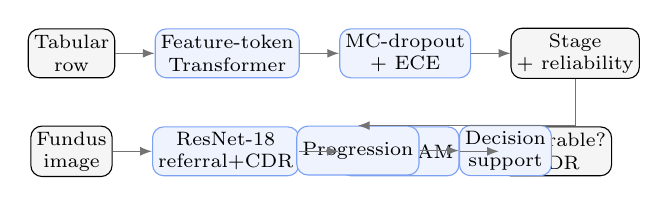
\begin{tikzpicture}[
  node distance=4mm and 5mm,
  box/.style={draw, rounded corners, align=center, font=\scriptsize,
              minimum height=6.2mm, inner sep=2pt, fill=accent!8, draw=accent!60},
  io/.style ={draw, rounded corners, align=center, font=\scriptsize,
              minimum height=6.2mm, inner sep=2pt, fill=black!4},
  ar/.style ={-{Latex[length=1.5mm]}, draw=black!55}
]
\node[io]  (tab) {Tabular\\row};
\node[box, right=of tab] (tf) {Feature-token\\Transformer};
\node[box, right=of tf]  (mc) {MC-dropout\\+ ECE};
\node[io,  right=of mc]  (st) {Stage\\+ reliability};
\node[io,  below=6mm of tab] (img) {Fundus\\image};
\node[box, right=of img] (cnn) {ResNet-18\\referral$+$CDR};
\node[box, right=of cnn] (cam) {Grad-CAM};
\node[io,  right=of cam] (ref) {Referable?\\CDR};
\node[box, below=6mm of mc, xshift=-6mm] (prog) {Progression};
\node[box, right=of prog] (dec) {Decision\\support};
\draw[ar] (tab)--(tf); \draw[ar] (tf)--(mc); \draw[ar] (mc)--(st);
\draw[ar] (img)--(cnn);\draw[ar] (cnn)--(cam);\draw[ar] (cam)--(ref);
\draw[ar] (st.south) |- (prog.north); \draw[ar] (prog)--(dec);
\end{tikzpicture}
\caption{System overview. Two modality-specific models feed transparent downstream
reasoning (progression projection and guideline decision support).}
\label{fig:arch}
\end{figure}

% ==================================================================
\section{System Implementation}
The backend is a FastAPI service (Table~\ref{tab:api}); the frontend is a minimal
React/Recharts dashboard that shows the stage, reliability flag, probability bars,
feature attributions, the progression chart, the decision-support card and the
Grad-CAM overlay---without decorative 3-D or animation that does not aid
interpretation. The fitted preprocessor and class metadata are persisted so training
and serving are bit-for-bit consistent.

\begin{table*}[t]
\centering
\caption{HTTP API. All endpoints are stateless and JSON (fundus is multipart).}
\label{tab:api}
\small
\begin{tabular}{lll}
\toprule
Endpoint & Input & Output \\
\midrule
\texttt{POST /predict} & feature dict, MC samples & stage, probabilities, confidence, reliability, attributions \\
\texttt{POST /simulate} & feature dict, horizon, IOP reduction & treated/untreated MD trajectory $+$ $80\%$ band \\
\texttt{POST /recommend-treatment} & feature dict & target IOP, at-target flag, next ladder step, rationale \\
\texttt{POST /analyze-fundus} & image (multipart) & referable flag, $p$(glaucoma), CDR, Grad-CAM, calibration flag \\
\texttt{GET /health} & --- & model and fundus-calibration status \\
\bottomrule
\end{tabular}
\end{table*}

% ==================================================================
\section{Results}
\label{sec:results}

\subsection{Aggregate staging performance}
On the held-out test set ($600$ patients) the model attains the metrics in
Table~\ref{tab:tabular}. ROC-AUC $0.954$ indicates strong ranking; ECE $0.108$ and
Brier $0.051$ indicate usable calibration, further improved by the reliability flag,
which abstains on high-uncertainty cases.

\begin{table}[t]
\centering
\caption{Aggregate test performance ($5$ classes, $N{=}600$).}
\label{tab:tabular}
\small
\begin{tabular}{lc}
\toprule
Metric & Value \\
\midrule
Accuracy & 0.843 \\ Macro-$F_1$ & 0.810 \\ ROC-AUC (OvR) & 0.954 \\
Brier score & 0.051 \\ ECE (15 bins) & 0.108 \\
\bottomrule
\end{tabular}
\end{table}

\subsection{Per-class analysis}
Table~\ref{tab:perclass} reports per-class precision/recall/$F_1$ and
Table~\ref{tab:cm} the confusion matrix. Performance is strongest for moderate,
severe and suspect ($F_1\ge0.87$) and weakest for \emph{mild} ($F_1{=}0.61$), whose
errors fall almost entirely into the neighbouring moderate and suspect classes. This
is clinically sensible: mild occupies the narrowest MD band ($-6$ to $-3\db$) and is
the genuine borderline category, so confusions are with adjacent stages rather than
catastrophic (e.g.\ no mild case is mistaken for severe).

\begin{table}[t]
\centering
\caption{Per-class test metrics (precision / recall / $F_1$ / support).}
\label{tab:perclass}
\small
\begin{tabular}{lcccc}
\toprule
Stage & P & R & $F_1$ & n \\
\midrule
Normal            & 0.822 & 0.789 & 0.805 & 76 \\
Suspect           & 0.894 & 0.874 & 0.884 & 261 \\
Mild Glaucoma     & 0.571 & 0.651 & 0.609 & 43 \\
Moderate Glaucoma & 0.868 & 0.874 & 0.871 & 143 \\
Severe Glaucoma   & 0.886 & 0.909 & 0.897 & 77 \\
\bottomrule
\end{tabular}
\end{table}

\begin{table}[t]
\centering
\caption{Confusion matrix (rows: true, columns: predicted).}
\label{tab:cm}
\small
\setlength{\tabcolsep}{4pt}
\begin{tabular}{l|ccccc}
\toprule
 & Mild & Mod & Norm & Sev & Susp \\
\midrule
Mild & \textbf{28} & 7 & 1 & 0 & 7 \\
Mod  & 6 & \textbf{125} & 0 & 8 & 4 \\
Norm & 1 & 0 & \textbf{60} & 0 & 15 \\
Sev  & 0 & 6 & 0 & \textbf{70} & 1 \\
Susp & 14 & 6 & 12 & 1 & \textbf{228} \\
\bottomrule
\end{tabular}
\end{table}

\subsection{Calibration}
Table~\ref{tab:rel} gives the reliability diagram. The model is mildly overconfident
in the $0.4$--$0.6$ range but well aligned at high confidence ($0.85$ confidence
$\rightarrow$ $0.92$ accuracy), where most mass lies; the global ECE is $0.108$.

\begin{table}[t]
\centering
\caption{Reliability diagram (test). conf $=$ mean confidence, acc $=$ empirical accuracy.}
\label{tab:rel}
\small
\begin{tabular}{cccc}
\toprule
bin & conf & acc & n \\
\midrule
$[0.4,0.5)$ & 0.462 & 0.593 & 27 \\
$[0.5,0.6)$ & 0.553 & 0.660 & 50 \\
$[0.6,0.7)$ & 0.658 & 0.759 & 83 \\
$[0.7,0.8)$ & 0.756 & 0.895 & 248 \\
$[0.8,0.9)$ & 0.851 & 0.921 & 190 \\
\bottomrule
\end{tabular}
\end{table}

\subsection{Fundus screening}
The fundus model converges to validation ROC-AUC $1.00$ with CDR MAE $\approx0.10$
(ACRIMA is comparatively separable). Qualitatively, on a held-out glaucomatous
photograph it returns referable glaucoma ($p{=}1.00$, estimated CDR $0.80$) with
Grad-CAM concentrated on the optic disc/cup and peripapillary rim, whereas a normal
photograph yields ``no referable glaucoma'' ($p{=}0.003$, CDR $0.41$). The
disc-centred saliency is evidence that the network attends to the clinically relevant
structure rather than spurious background.

\subsection{Ablation: bounding the aleatoric term}
\label{sec:ablation}
With the \emph{unbounded} variance term and loss-based checkpointing, training loss
diverged to large negative values and test accuracy collapsed to $0.45$
(macro-$F_1$ $0.47$) despite ROC-AUC $\approx0.90$---the representation was fine but
the argmax was corrupted. Clamping $\sigma^2$ to $[0,1]$ and selecting on macro-$F_1$
raised accuracy to $0.843$ and macro-$F_1$ to $0.810$
(Table~\ref{tab:ablation}). The decisive gain came from removing a single,
clinically irrelevant numerical pathology---a reminder that auxiliary
uncertainty objectives must be bounded.

\begin{table}[t]
\centering
\caption{Ablation of the aleatoric term and checkpoint metric.}
\label{tab:ablation}
\small
\begin{tabular}{lccc}
\toprule
Configuration & Acc & Macro-$F_1$ & AUC \\
\midrule
Unbounded $\sigma^2$, ckpt on loss & 0.45 & 0.47 & 0.90 \\
Bounded $\sigma^2$, ckpt on $F_1$  & \textbf{0.843} & \textbf{0.810} & \textbf{0.954} \\
\bottomrule
\end{tabular}
\end{table}

% ==================================================================
\section{Discussion, Limitations and Ethics}
The system's headline property is \emph{auditability}: labels follow a published
staging rule, the progression and treatment modules are closed-form and disclosed,
uncertainty is shown rather than hidden, and the fundus model declares when it is
uncalibrated. We see this transparency as a precondition for clinical trust.

\textbf{Limitations.} (i)~The tabular cohort is \emph{synthetic}; absolute metrics
reflect the generator's structure and must be re-established on real, multi-site data.
(ii)~The design is \emph{cross-sectional}; genuine progression modeling requires
longitudinal records and would replace the closed-form projector with a fitted
mixed-effects or state-space model. (iii)~The fundus CDR target is \emph{synthetic},
so the CDR output is an indicative structural estimate that partly tracks the
diagnosis; only the binary referral output is trained on real labels. (iv)~ACRIMA is
single-source, so the reported AUC will not transfer unchanged across cameras and
populations; external validation (e.g.\ REFUGE, G1020) is required.
(v)~The weakest class (mild) reflects an intrinsically narrow decision band; cost-
sensitive training or ordinal regression may help.

\textbf{Ethics.} This is a research and educational artifact, not a medical device,
and must not be used for patient care. Every recommendation is advisory and defers to
the treating ophthalmologist; the data are synthetic and contain no patient
information.

% ==================================================================
\section{Conclusion}
We described a glaucoma decision-support system rebuilt around clinical reasoning:
rule-derived staging, uncertainty-aware tabular prediction with explicit reliability,
transparent progression and treatment guidance, and an honest fundus screener. A
detailed evaluation---aggregate, per-class, calibration and ablation---shows that
removing clinically invalid machinery and correcting a single numerical pathology
yields a system that is simultaneously more trustworthy and more accurate. All code,
data generators and trained weights are released to support reproduction and
critique.

% ==================================================================
\section*{Reproducibility}
The repository provides \texttt{generate\_synthetic\_data.py},
\texttt{fetch\_fundus\_dataset.py}, \texttt{augment\_fundus\_cdr.py},
\texttt{train\_fundus.py}, the train/serve entrypoint \texttt{run.py}, and the
dashboard. Tabular results use seed $42$; the held-out split is deterministic.

% ==================================================================
\begin{thebibliography}{9}
\small
\bibitem{hpa} E.~Hodapp, R.~K.~Parrish, D.~R.~Anderson.
\textit{Clinical Decisions in Glaucoma.} Mosby, 1993.
\bibitem{emgt} M.~C.~Leske \textit{et al.}
``Factors for glaucoma progression and the effect of treatment: the Early Manifest
Glaucoma Trial.'' \textit{Arch. Ophthalmol.}, 2003.
\bibitem{cigts} P.~R.~Lichter \textit{et al.}
``Interim clinical outcomes in the CIGTS comparing initial treatment randomized to
medications or surgery.'' \textit{Ophthalmology}, 2001.
\bibitem{agis} ``The AGIS: the relationship between control of IOP and visual field
deterioration.'' \textit{Am. J. Ophthalmol.}, 2000.
\bibitem{acrima} A.~Diaz-Pinto \textit{et al.}
``CNNs for automatic glaucoma assessment using fundus images: an extensive
validation.'' \textit{BioMed. Eng. OnLine}, 2019.
\bibitem{resnet} K.~He \textit{et al.}
``Deep residual learning for image recognition.'' \textit{CVPR}, 2016.
\bibitem{transformer} A.~Vaswani \textit{et al.}
``Attention is all you need.'' \textit{NeurIPS}, 2017.
\bibitem{mcdropout} Y.~Gal, Z.~Ghahramani.
``Dropout as a Bayesian approximation: representing model uncertainty in deep
learning.'' \textit{ICML}, 2016.
\bibitem{gradcam} R.~R.~Selvaraju \textit{et al.}
``Grad-CAM: visual explanations from deep networks via gradient-based
localization.'' \textit{ICCV}, 2017.
\bibitem{shap} S.~Lundberg, S.-I.~Lee.
``A unified approach to interpreting model predictions.'' \textit{NeurIPS}, 2017.
\bibitem{refuge} J.~I.~Orlando \textit{et al.}
``REFUGE Challenge: evaluating automated methods for glaucoma assessment from fundus
photographs.'' \textit{Med. Image Anal.}, 2020.
\bibitem{ece} C.~Guo \textit{et al.}
``On calibration of modern neural networks.'' \textit{ICML}, 2017.
\end{thebibliography}

\end{document}
